%!TEX program = xelatex

\documentclass[12pt]{beamer}
\usepackage{graphicx}

\setlength{\parindent}{0pt}

%\setbeameroption{show notes}
\makeatletter
\def\beamer@framenotesbegin{% at beginning of slide
    \gdef\beamer@noteitems{}%
    \gdef\beamer@notes{{}}% used to be totally empty.
}
\makeatother

% Theme stuff
% -----------
\usetheme{default}
\beamertemplatenavigationsymbolsempty
\setbeamertemplate{itemize items}[circle]
\setbeamertemplate{enumerate items}[default]
\setbeamercolor{enumerate item}{fg=black}
%\setbeamertemplate{footline}[frame number]

% Font stuff
% ----------
\usepackage[no-math]{fontspec}
\defaultfontfeatures{Mapping=tex-text}
\setsansfont[BoldFont=P22UndergroundBook,
			 SmallCapsFont=P22UndergroundLightSC]{P22UndergroundLight}
\setmonofont{Hack}



% Define colors
% -------------
\usepackage{xcolor}
\definecolor{BGDarkGrey}{RGB}{50,50,50}
\definecolor{BGBlue}{RGB}{77,143,249}
\definecolor{LightGrey}{RGB}{200,200,200}
\definecolor{Grey50}{RGB}{128,128,128}
\definecolor{LBlue}{HTML}{29B6F6}
\definecolor{Blue}{HTML}{42A5F5}
\definecolor{Orange}{HTML}{FFA726}
\definecolor{LGreen}{HTML}{9CCC65}
\definecolor{Green}{HTML}{66BB6A}
\definecolor{Red}{HTML}{EF5350}
\definecolor{Amber}{HTML}{FFCA28}
\definecolor{Yellow}{HTML}{FFEE58}
\definecolor{Cyan}{HTML}{26C6DA}
\definecolor{Indigo}{HTML}{5C6BC0}
\definecolor{Lime}{HTML}{D4E157}
\definecolor{BlueGrey}{HTML}{78909C}
\definecolor{DeepOrange}{HTML}{FF7043}
\definecolor{Grey}{HTML}{424242}
\definecolor{Teal}{HTML}{26A69A}

\definecolor{DhakaBlue}{RGB}{102,167,221}
\definecolor{WikiGrey}{RGB}{252,252,252}

\renewcommand{\arraystretch}{2}

% Table package
% -------------
\usepackage{booktabs}

% Background
% ----------
\usepackage{tikz}

\begin{document}


% Title
\setbeamercolor{normal text}{fg=Grey, bg=white}
\usebeamercolor[fg]{normal text}
\begin{frame}

	\null
	\vfill
	%\centering
	\textcolor{black}{\textsc{\large A Comparative Study of Techniques for Estimation and Inference of Nonlinear Stochastic Time Series}} \\
	\vspace{1.5\baselineskip}
	\noindent\textcolor{black}{\rule{\textwidth}{0.4pt}} \\
	\vspace{2\baselineskip}
	Dexter Barrows, B.Sc. \\
	\vspace{1\baselineskip}
	Masters Thesis Defence \\
	McMaster University \\
	April 2016
	\vfill

\end{frame}


% Authors
\setbeamercolor{normal text}{fg=Grey, bg=white}
\usebeamercolor[fg]{normal text}
\begin{frame}

	\vspace{\baselineskip}
	\begin{columns}
		\begin{column}{0.8\textwidth}
			{\large
			\begin{enumerate}
				\item Framing
				\item Hamiltonian HMCMC
				\item Iterated Filtering 2
				\item Model Fitting
				\item Forecasting Frameworks
				\item S-maps \& Seasonal Outbreaks
				\item Spatiotemporal Epidemics
				\item Parallelism \& Future Directions
			\end{enumerate}
			}
		\end{column}
	\end{columns}

\end{frame}

%% 1. INTRODUCTION
%% --------------------------------------------------------------------------------------
%% --------------------------------------------------------------------------------------

% Section title
\setbeamercolor{normal text}{fg=white, bg=BGBlue}
\usebeamercolor[fg]{normal text}
\begin{frame}

	\vspace{2cm}
	\hspace{2.5cm} {\Huge Framing }
	\begin{tikzpicture}[overlay]
	    \node[at=(current page.center), shift={(-4.5 cm, -4.7 cm)}, opacity=0.25] {
	    	\fontsize{200pt}{0pt}\selectfont
	        \color{white}{1}
	    };
	\end{tikzpicture}

\end{frame}

\setbeamercolor{normal text}{fg=Grey, bg=white}
\usebeamercolor[fg]{normal text}
\begin{frame}

	Some stuff about forecasting being important ... \\
	... and lacking a ``gold standard''

\end{frame}


%% 2. HMCMC
%% --------------------------------------------------------------------------------------
%% --------------------------------------------------------------------------------------

% Section title
\setbeamercolor{normal text}{fg=white, bg=Green}
\usebeamercolor[fg]{normal text}
\begin{frame}

	\vspace{2cm}
	\hspace{0cm} {\Huge Hamiltonian MCMC }
	\begin{tikzpicture}[overlay]
	    \node[at=(current page.center), shift={(-5 cm, -4.7 cm)}, opacity=0.25] {
	    	\fontsize{200pt}{0pt}\selectfont
	        \color{white}{2}
	    };
	\end{tikzpicture}

\end{frame}

\setbeamercolor{normal text}{fg=Grey, bg=white}
\usebeamercolor[fg]{normal text}
\begin{frame}

	It's coooollllll.... it has physiiiiicccsssssss

\end{frame}


%% 3. IF2
%% --------------------------------------------------------------------------------------
%% --------------------------------------------------------------------------------------

% Section title
\setbeamercolor{normal text}{fg=white, bg=Red}
\usebeamercolor[fg]{normal text}
\begin{frame}

	\vspace{2cm}
	\hspace{0cm} {\Huge Iterated Filtering 2 }
	\begin{tikzpicture}[overlay]
	    \node[at=(current page.center), shift={(-4.5 cm, -4.7 cm)}, opacity=0.25] {
	    	\fontsize{200pt}{0pt}\selectfont
	        \color{white}{3}
	    };
	\end{tikzpicture}

\end{frame}

\setbeamercolor{normal text}{fg=Grey, bg=white}
\usebeamercolor[fg]{normal text}
\begin{frame}

	Didn't we skip a step????

\end{frame}


%% 4. Model Fitting
%% --------------------------------------------------------------------------------------
%% --------------------------------------------------------------------------------------

% Section title
\setbeamercolor{normal text}{fg=white, bg=Amber}
\usebeamercolor[fg]{normal text}
\begin{frame}

	\vspace{2cm}
	\hspace{0.5cm} {\Huge Model Fitting }
	\begin{tikzpicture}[overlay]
	    \node[at=(current page.center), shift={(-3.8 cm, -4.7 cm)}, opacity=0.25] {
	    	\fontsize{200pt}{0pt}\selectfont
	        \color{white}{4}
	    };
	\end{tikzpicture}

\end{frame}

% Basic Stochastic SIR
\setbeamercolor{normal text}{fg=white, bg=Grey}
\setbeamercolor{footline}{parent=normal text}
\usebeamercolor[fg]{normal text}
\begin{frame}

	\null
	{\large \textcolor{Cyan}{Stochastic SIR Model}}
	\vfill

	\centering
	\begin{align*}
		\dfrac{dS}{dt} 	& = - \beta S I \\
		\dfrac{dI}{dt} 	& = \beta S I - \gamma I \\
		\dfrac{dR}{dt} 	& =  \gamma I
	\end{align*}
	\vspace{0.5\baselineskip}
	$+$	\\
	\vspace{1\baselineskip}
	$\beta_{i+1} = \exp \left[ \beta_i + \eta \left( \bar{\beta} - \beta_i  \right) + \mathcal{N}(0, \sigma_{\small\text{proc}}) \right]$

\end{frame}

\setbeamercolor{normal text}{fg=Grey, bg=white}
\usebeamercolor[fg]{normal text}
\begin{frame}

	\null
	\vfill
	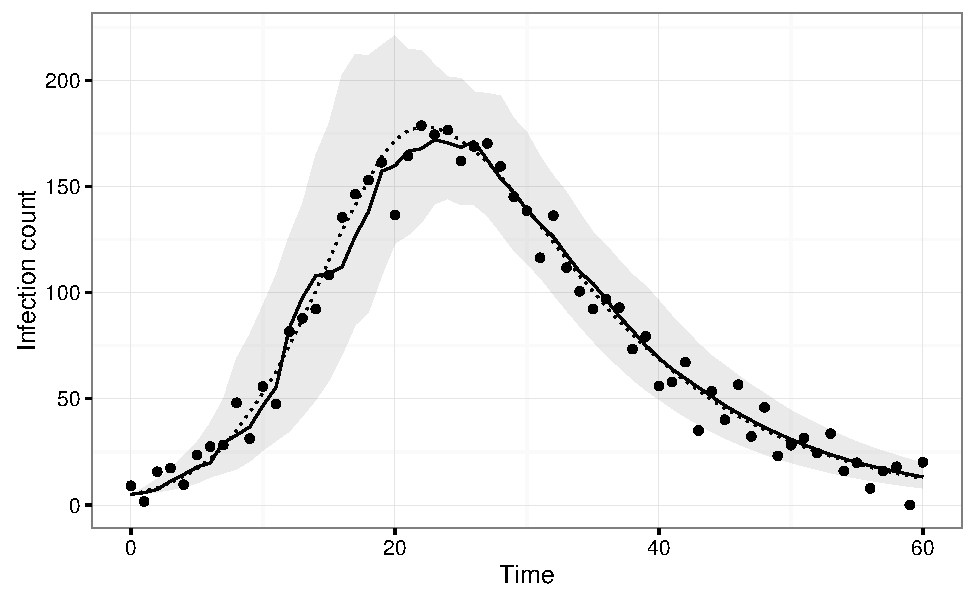
\includegraphics[width=\textwidth,height=\textheight,keepaspectratio=true]{../../writing/SC1/images/sirmean}
	\vfill

\end{frame}

\setbeamercolor{normal text}{fg=Grey, bg=white}
\usebeamercolor[fg]{normal text}
\begin{frame}

	Mmmmm, Kernels

\end{frame}

%% 5. Forecasting Frameworks
%% --------------------------------------------------------------------------------------
%% --------------------------------------------------------------------------------------

% Section title
\setbeamercolor{normal text}{fg=white, bg=Cyan}
\usebeamercolor[fg]{normal text}
\begin{frame}

	\vspace{2cm}
	\hspace{1cm} {\Huge Forecasting } \\
	\hspace{1cm} {\Huge Frameworks }
	\begin{tikzpicture}[overlay]
	    \node[at=(current page.center), shift={(-4 cm, -4.3 cm)}, opacity=0.25] {
	    	\fontsize{200pt}{0pt}\selectfont
	        \color{white}{5}
	    };
	\end{tikzpicture}

\end{frame}

\setbeamercolor{normal text}{fg=Grey, bg=white}
\usebeamercolor[fg]{normal text}
\begin{frame}

	Fuzzy bootstrapping

\end{frame}


%% 6. S-maps and SIRS
%% --------------------------------------------------------------------------------------
%% --------------------------------------------------------------------------------------

% Section title
\setbeamercolor{normal text}{fg=white, bg=Indigo}
\usebeamercolor[fg]{normal text}
\begin{frame}

	\vspace{2cm}
	\hspace{-0.5cm} {\Huge S-maps \& } \\
	%\vspace{0.05cm}
	\hspace{-0.5cm} {\Huge Seasonal Outbreaks }
	\begin{tikzpicture}[overlay]
	    \node[at=(current page.center), shift={(-4.7 cm, -4.3 cm)}, opacity=0.25] {
	    	\fontsize{200pt}{0pt}\selectfont
	        \color{white}{6}
	    };
	\end{tikzpicture}

\end{frame}

% SIRS
\setbeamercolor{normal text}{fg=white, bg=Grey}
\setbeamercolor{footline}{parent=normal text}
\usebeamercolor[fg]{normal text}
\begin{frame}

	\null
	{\large \textcolor{Cyan}{Stochastic SIRS Model}}
	\vfill

	\centering
	\begin{align*}
		\dfrac{dS}{dt} 	& = - \beta S I + \textcolor{Teal}{\alpha R}\\
		\dfrac{dI}{dt} 	& = \beta S I - \gamma I \\
		\dfrac{dR}{dt} 	& =  \gamma I - \textcolor{Teal}{\alpha R}
	\end{align*}
	\vspace{0.5\baselineskip}
	$+$	\\
	\vspace{1\baselineskip}
	$\beta_{i+1} = \exp \left[ \beta_i + \eta \left( \bar{\beta} - \beta_i  \right) + \mathcal{N}(0, \sigma_{\small\text{proc}}) \right]$

\end{frame}

\setbeamercolor{normal text}{fg=Grey, bg=white}
\usebeamercolor[fg]{normal text}
\begin{frame}

	\null
	\vfill
	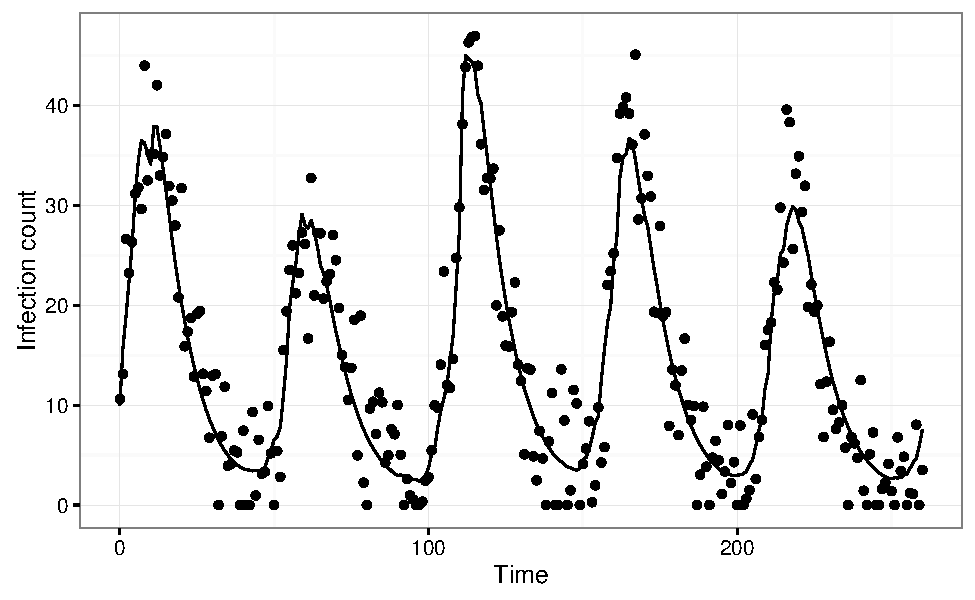
\includegraphics[width=\textwidth,height=\textheight,keepaspectratio=true]{../../writing/SIRS-SMAP/images/dataplot}
	\vfill

\end{frame}

\setbeamercolor{normal text}{fg=Grey, bg=white}
\usebeamercolor[fg]{normal text}
\begin{frame}

	Sugihara in the hizzy, knowahtimsaying????

\end{frame}


%% 7. Spatiotemporal
%% --------------------------------------------------------------------------------------
%% --------------------------------------------------------------------------------------

% Section title
\setbeamercolor{normal text}{fg=white, bg=BlueGrey}
\usebeamercolor[fg]{normal text}
\begin{frame}

	\vspace{2cm}
	\hspace{0cm} {\Huge Spatiotemporal } \\
	\vspace{0.1cm}
	\hspace{0cm} {\Huge Epidemics }
	\begin{tikzpicture}[overlay]
	    \node[at=(current page.center), shift={(-2 cm, -4.2 cm)}, opacity=0.25] {
	    	\fontsize{200pt}{0pt}\selectfont
	        \color{white}{7}
	    };
	\end{tikzpicture}

\end{frame}

\setbeamercolor{normal text}{fg=Grey, bg=white}
\usebeamercolor[fg]{normal text}
\begin{frame}

	If you liked it then you should have put a ring on it

\end{frame}



%% 8. Parallelism and FUture Directions
%% --------------------------------------------------------------------------------------
%% --------------------------------------------------------------------------------------

% Section title
\setbeamercolor{normal text}{fg=white, bg=DeepOrange}
\usebeamercolor[fg]{normal text}
\begin{frame}

	\vspace{2cm}
	\hspace{0cm} {\Huge Parallelism \& } \\
	\vspace{0.3cm}
	\hspace{0cm} {\Huge Future Directions }
	\begin{tikzpicture}[overlay]
	    \node[at=(current page.center), shift={(-4.7 cm, -4.3 cm)}, opacity=0.25] {
	    	\fontsize{200pt}{0pt}\selectfont
	        \color{white}{8}
	    };
	\end{tikzpicture}

\end{frame}

\setbeamercolor{normal text}{fg=Grey, bg=white}
\usebeamercolor[fg]{normal text}
\begin{frame}

	More than Moore

\end{frame}


\end{document}